\documentclass[journal,10pt,twocolumn]{article}
\usepackage{graphicx, float}
\usepackage[margin=0.5in]{geometry}
\usepackage{amsmath, bm}
\usepackage{array}
\usepackage{booktabs}

\providecommand{\norm}[1]{\left\lVert#1\right\rVert}
\let\vec\mathbf
\newcommand{\myvec}[1]{\ensuremath{\begin{pmatrix}#1\end{pmatrix}}}
\newcommand{\mydet}[1]{\ensuremath{\begin{vmatrix}#1\end{vmatrix}}}

\title{\textbf{Conics Assignment}}
\author{Pallavarapu Sravan kumar}
\date{October 2022}

\begin{document}

\maketitle
\paragraph{\textit{\large Problem Statement} -If two tangents drawn from a point P to the parabola y$^2$=4x are at right angles, then the locus of P is}
\section*{\large Solution}
\begin{figure}[H]
\centering
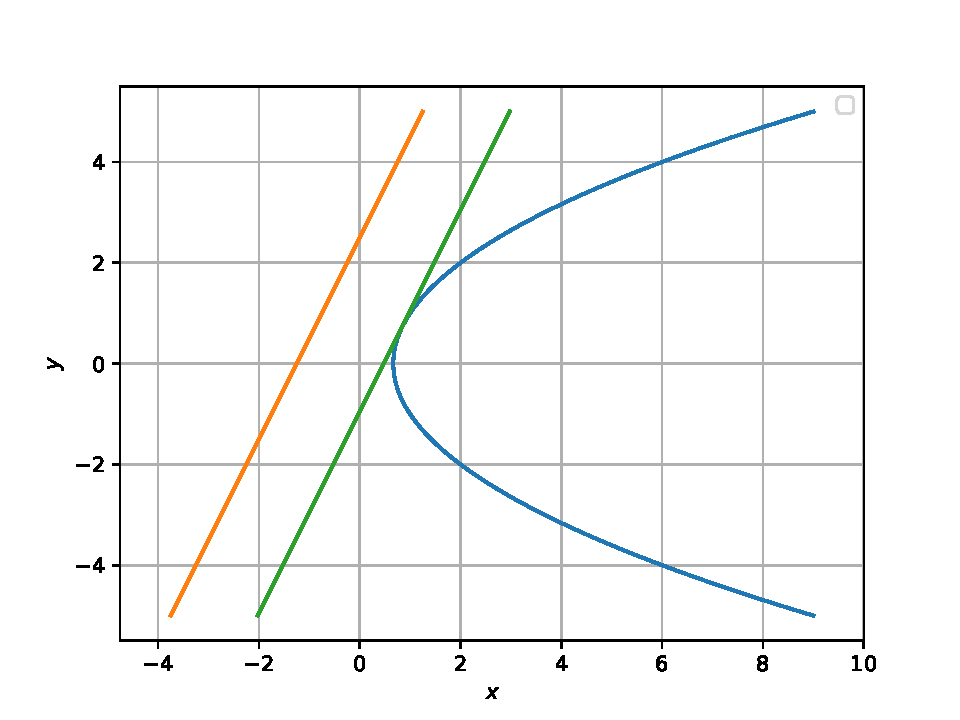
\includegraphics[width=1\columnwidth]{conic.pdf}
\caption{}
\end{figure}

\section*{\large Construction}

\begin{table}[htbp]
 \begin{center}
    \begin{tabular}{|l|c|c|c|c|c|c} \hline \textbf{Symbol}
  & \textbf{value} & \textbf{Description} \\
 \hline
V &\myvec{0\\0} & Vertex of parabola\\ \hline
F&\myvec{-2\\0} & focus of parabola\\ \hline
n &\myvec{1\\0}   & normal of directrix\\ \hline

	
\end{tabular}   
\end{center}
\caption{\label{table:dummytable} }
\end{table}



\section*{Proof:}


The given equation of parabola $y^2 = 4x$ can be written in the general quadratic form as
\begin{align}
    \label{eq:conic_quad_form}
    \vec{x}^{\top}\vec{V}\vec{x}+2\vec{u}^{\top}\vec{x}+f=0
    \end{align}

where:
\begin{align}
	\label{eq:V_matrix}
	\vec{V} &= \myvec{0 & 0\\0 & 1},
	\\
	\label{eq:u_vector}
	\vec{u} &= \myvec{-2\\0},
	\\
	\label{eq:f_value}
	f &= 0
	%\\
\end{align}

let vector point $\vec{P}$ as $\vec{h}$
where:
\begin{eqnarray*}
\vec{h}=\myvec{k\\l}
\end{eqnarray*}
Given two tangents from  point $\vec{h}$ make right angles with the parabola.The normal vectors of the tangents from a point $\vec{h}$ to the conic are given by
\begin{eqnarray}
\vec{n}=\frac{\vec{e1}}{\vec{e1}^T\vec{h}}+\mu_i \vec{R}\vec{h}
\end{eqnarray}
\vspace*{10mm}
where:

 \begin{eqnarray*}
	\vec{R}=\myvec{0 & -1 \\ 1 & 0} &  \vec{e1}=\myvec{1 \\ 0}
\end{eqnarray*}
 
By substituting 
\begin{eqnarray}
	\vec{n}=\myvec{\frac{1}{k}-\mu_i{l} \\ \mu_i k}
\end{eqnarray}


where:

\begin{multline*}
\vec{\mu_i}=\\
\frac{-\vec{m}^T(\vec{V}\vec{q}+\vec{u})\pm \sqrt{(\vec{m}^T(\vec{V}\vec{q}+\vec{u}))^2-(\vec{q}^T\vec{V}\vec{q}+2\vec{u}^T\vec{q}+f)\vec{m}^T\vec{V}\vec{m}}}{\vec{m}^T\vec{V}\vec{m}}
\end{multline*}


for $\mu_i$ substitute:

\begin{eqnarray*}
	\vec{m}=\vec{R}\vec{h}=\myvec{-l\\k}& \vec{u}=\myvec{-2\\0}
\end{eqnarray*}

\begin{eqnarray*}
	\vec{q}=\frac{\vec{e1}}{\vec{e1}^T\vec{h}}=\myvec{\frac{1}{k} \\ 0}
\end{eqnarray*}

\begin{eqnarray*}
	\vec{V}=\vec{V}^{-1}= \myvec{1 & 0 \\ 0 & 0}
\end{eqnarray*}

By substituting 
\begin{eqnarray*}
	\vec{\mu_1}=\frac{1}{kl} & \vec{\mu_2}=\frac{1}{l}(\frac{1}{k}+4)
\end{eqnarray*}


By substituting $\mu$ values in (6)

\begin{eqnarray}
	\vec{n_1}=\myvec{0 \\ \frac{1}{l}}
\end{eqnarray}

\begin{eqnarray}
	\vec{n_2}=\myvec{-4 \\ \frac{1}{l}(\frac{1}{k}+4)}
\end{eqnarray}



Since the two tangents are perpendicular
\begin{eqnarray*}
	\vec{n_1^T}\vec{n_2}=0
\end{eqnarray*}

\begin{eqnarray*}
	\myvec{0 \ & \frac{1}{l}}\myvec{-4 \\ \frac{1}{l}(\frac{1}{k}+4)}=0
\end{eqnarray*}

\begin{eqnarray}
	k=\frac{-1}{4}
\end{eqnarray}

By substituting k value in (8)
\begin{eqnarray}
\vec{n_2}=\myvec{-4 \\ 0}
\end{eqnarray}
Since the tangent2 pass through the point h
\begin{eqnarray*}
\vec{n_2}^T\vec{h}=0
\end{eqnarray*}

\begin{eqnarray}
\myvec{-4 \ & 0} \myvec{k \\ l} = 1
\end{eqnarray}

 
\end{document}
